\documentclass{article}

\usepackage{mhchem} % Package for chemical equation typesetting
\usepackage{siunitx} % Provides the \SI{}{} command for typesetting SI units
\usepackage{pdfsync}
\usepackage[english]{babel}
\usepackage{fullpage}
\usepackage{amsmath}
\usepackage[table]{xcolor}
\usepackage{multirow}
\usepackage{graphicx}
\usepackage{circuitikz}
\usepackage{caption}
\usepackage{subcaption}
\usepackage{float}
\usepackage{verbatim}
\usepackage{eso-pic}
\usepackage[toc,page]{appendix}
\usepackage[linkbordercolor={white}]{hyperref}
\usepackage{nameref}
\usepackage{listings}
\usepackage{graphicx} % Required for the inclusion of images

\setlength\parindent{0pt} % Removes all indentation from paragraphs

\lstdefinestyle{custommcrl2}{%
  belowcaptionskip=1\baselineskip,
  xleftmargin=\parindent,
  basicstyle=\footnotesize\ttfamily
}


%----------------------------------------------------------------------------------------
%	TITLE AND DOCUMENT INFORMATION
%----------------------------------------------------------------------------------------
\begin{document}

\centering
\vspace{+150pt}
\LARGE{Report System Validation Project \\
  Modeling a Bridge Control System\\
  Creating a safety layer with mCRL2 using Labelled Transition Systems} % Title
\vspace{+50pt} % Ruimte tussen titel en auteurs

\Large{Aimee \textsc{Ferouge} 4014030 \\
  Wieger \textsc{IJntema} 4034570 \\
  Arian \textsc{Stolwijk} 4001079 \\
  Group 7} % Author name

\vspace{+50pt} % Title
\today % Date for the report
\vspace{+300pt} % Title

\vfill
\begin{center}
\begin{tabular}{l r}
Date Performed: & Januari, 2013 \\ % Date the experiment was performed
Instructor: & J. J. A. Keiren % Instructor/supervisor
\end{tabular}
\end{center}

\raggedright
\normalsize


%----------------------------------------------------------------------------------------
%	Preface, lists, TOC
%----------------------------------------------------------------------------------------

\pagenumbering{roman}
\setcounter{page}{0}

\addcontentsline{toc}{section}{Preface}
\newpage
\section*{Preface}

This document holds a report describing our foundings during the project of System Validaton, course IN4387 of the Embedded Systems master.
The topic of the assigment is to
%
\begin{enumerate}
	\item designing a safety control layer for a bridge system and
	\item checking whether all safety requirements are satisfied by the model.
\end{enumerate}
%
As this is just a draft of the final report, we would like to acknowledge the fact that perhaps the report is still to be improved. Also, the model is still very simple. In the next two weeks, we will attempt to add more detail to the model.

Hopefully you will enjoy this report. In case of any questions, we would be happy to answer them. Just send an email to one of us.\\
\vspace{+50pt}
Aimee Ferouge\\
Wieger IJntema\\
Arian Stolwijk


\newpage
\addcontentsline{toc}{section}{List of Figures}
\listoffigures
\addcontentsline{toc}{section}{List of Tables}
\listoftables

\newpage
\tableofcontents
\newpage
\pagestyle{plain}
\pagenumbering{arabic}
\setcounter{page}{1}
\setcounter{section}{0}

%\addcontentsline{toc}{section}{Summary}
%\section*{Summary}

Bla.


\newpage

%----------------------------------------------------------------------------------------
%	Report
%----------------------------------------------------------------------------------------
%\section*{Summary}

Bla.


\newpage
\subsection{Introduction}

As has been pointed out by the incident at the Ketelbrug between Emmeloord and Lelystad, bridges require a very precise control system.  Many examples exist where bridges are not opened or closed properly, where bridge components break down or the bridge is being stuck in a particular state. The goal of this project is to design a satefy layer that can be added to the main control interface, in order to capture all possible situations and failures.
Throughout the report, we make use of the following assumptions:
%
\begin{itemize}
	\item If three or four sensors detect an open/closed bridge, the bridge can be considered open/closed
	\item If only the four sensor have a 50/50 detection on the bridge deck, the bridge should remain in its current position (open/closed)
	\item A barrier can only be considered to be down when the majority of the sensors detect a lowered barrier
\end{itemize}
%
In this section, the desired behaviour of the bridge is being determinated and defined. Section \ref{sec:glob} contains the global requirements that will be met in our system. Specific interactions that can be performed by the bridge are discussed in Section \ref{sec:act}, whereas Section \ref{sec:trans} translates these interactions into the requirements stated earlier.

\subsection{Global Requirements}
\label{sec:glob}

Using the Project Guide\footnote{J. J. A. Keiren, System Validation (IN4387) Project Guide, VU University Amterdam, november 2013} as a source for the desired behaviour, the following requirements are defined:
\\
\\
\textbf{Opening the bridge}
	\begin{enumerate}
  	\item Switching on pre signs should be the first action when opening the bridge
		\item Stop signs cannot be lit as long as the pre lights have not been lit
		\item Barriers cannot be lowered if the stop signs have not been lit
		\item Bridge can only be unlocked when all barriers are down
		\item The deck can only lifted when both locks are unlocked
   \newcounter{enumTemp}
   \setcounter{enumTemp}{\theenumi}
 \end{enumerate}

\textbf{Closing the bridge}
  \begin{enumerate}
    \setcounter{enumi}{\theenumTemp}
  	\item Bridge can only be locked when the deck is down
		\item Barriers can only be up when the bridge is locked by at least
		\setcounter{enumTemp}{\theenumi}
  \end{enumerate}

\textbf{Functional requirements}
	\begin{enumerate}

			\item The bridge should be able to be opened when a ship approaches
			\item The bridge should be able to close in order to let cars pass
			\item The first barrier to be encountered by the cars is lowered earlier than the second in order to enable cars to leave the bridge
		\setcounter{enumTemp}{\theenumi}
	\end{enumerate}

\textbf{Failure}
	\begin{enumerate}
		\setcounter{enumi}{\theenumTemp}
			\item The stop signs can only be lit if at least one pre signs is being lit at each side of the bridge
			\item The barriers can only be lowered if both stop signs are being lit at each side of the bridge
			\item If the motor is in the 'broken' status, the bridge may not be opened
		\setcounter{enumTemp}{\theenumi}
	\end{enumerate}

\subsection{Interactions}
\label{sec:act}

The interactions can be divided into two categories. The first category contains the global interactions, which are the direct translations of the requirements from Section \ref{sec:glob}.
Switching of the signs, moving the barriers or engaging the locking pins are all action to be performed by the controller and can be found in Table \ref{tab:glob_act}
The internal interactions are used for communication purposes, combining the state perceptions of different processes. These can be found in Table \ref{tab:int_act}
%
\begin{table}[htb]%
\begin{tabular}{lll}
      \textbf{Interaction} &	\textbf{Descripton}	&	\textbf{Parameters}\\
      \hline
      \mcode{openBridge} & Initiates the system to open the bridge &\\
      \mcode{closeBridge} & Initiates the system to close the bridge & \\
      \mcode{setPre} & Switches on/off the pre sign & Sign, signStatus\\
      \mcode{setStop} & Switches on/off the stop sign & Sign, signStatus\\
      \mcode{setBarrier} & Lifts/lowers the barriers & Barrier, barrierStatus\\
      \mcode{setLock} & Engages/disengages the locks & Lock, lockStatus\\
      \mcode{setDeck} & Lifts/lowers the bridge deck & Deck, deckStatus\\
\end{tabular}
\caption{All global interactions to be performed by the safety layer of the control system.}
\label{tab:glob_act}
\end{table}

\begin{table}[htb]%
\begin{tabular}{lll}
      \textbf{Interaction} &	\textbf{Description}	&	\textbf{Parameters}\\
      \hline
      \mcode{sendPre} & Sends the status of a particular pre signs & Sign, signStatus\\
      \mcode{receivePre} & Receives status of a particular pre signs & Sign, signStatus\\
      \mcode{commPreSign} & Synchronization action for sendPre $\mid$ receivePre &\\
      
      \mcode{sendStop} & Sends the status of a particular stop sign & Sign, signStatus\\
      \mcode{receiveStop} & Receives status of a particular stop signs & Sign, signStatus\\
      \mcode{commStopSign} & Synchronization action for sendStop $\mid$ receiveStop &\\
      
      \mcode{sendBarrier} & Sends the status of a particular barrier & Barrier, barrierStatus\\
      \mcode{receiveBarrier} & Receives status of a particular barrier & Barrier, barrierStatus\\
      \mcode{commBarrier} & Synchronization action for sendBarrier $\mid$ receiveBarrier &\\
      
      \mcode{sendLock} & Sends the status of a locking pin & Lock, lockStatus\\
      \mcode{receiveLock} & Receives status of a particular locking pin & Lock, lockStatus\\
      \mcode{commLock} & Synchronization action for sendLock $\mid$ receiveLock &\\
      
      \mcode{sendDeck} & Sends the status of the bridge deck & deckStatus\\
      \mcode{receiveDeck} & Receives status of the bridge deck & deckStatus\\
      \mcode{commDeck} & Synchronization action for sendDeck $\mid$ receiveDeck &\\
      
      \mcode{motorStatus} & Receives the status of the motor & Status\\
\end{tabular}
\caption{All internal interactions of the safety layer of the control system.}
\label{tab:int_act}
\end{table}

For the values of the interactions, datatypes are introduced which group certain values. Table \ref{tab:types} lists these datatypes and their possible values.

\begin{table}[htb]%
\begin{tabular}{lll}
	\textbf{Datatype} & \textbf{Values}\\
	Sign & P1, P2, P3, P4, S1, S2, S3, S4\\
	signStatus & on, off\\
	barrierStatus & up, down\\
	lockStatus & engage, disengage\\
	deckStatus & up, down\\
\end{tabular}
\caption{Datatypes used as parameters for the interactions.}
\label{tab:types}
\end{table}
\newpage
\section{Architecture}
\label{sec:arch}

Three parallel processes exist being \emph{signs}, \emph{barriers} and \emph{bridge}. \emph{Signs} handles the control of the lights, whereas \emph{barriers} handles the barriers and \emph{bridge} the locks and the deck.

\emph{Signs} is the first one to be executed when an \texttt{open} or \texttt{close} command is given. After first lighting the pre signs and then the stop signs, control is given to the \emph{barriers} process.

\emph{Barriers} makes sure all barriers are lowered if the stop signs are lit. When this is the case, \emph{bridge} takes over.

\emph{Bridge} handles the lifting and lowering of the bridge deck. Only when all barriers are down, the two locks of the bridge are disengaged and the deck can be moved up and down. When finishing this movement, control is given back first to \emph{barriers} and finally back to \emph{barriers}.

Figure \ref{fig:arch} shows a diagram of the communication flow between these parallel processes. As you can see, also the global actions that are available to the bridge operator are included. They are pictured as italic actions from outside the system.
%
\begin{figure}[htb]%
\centering
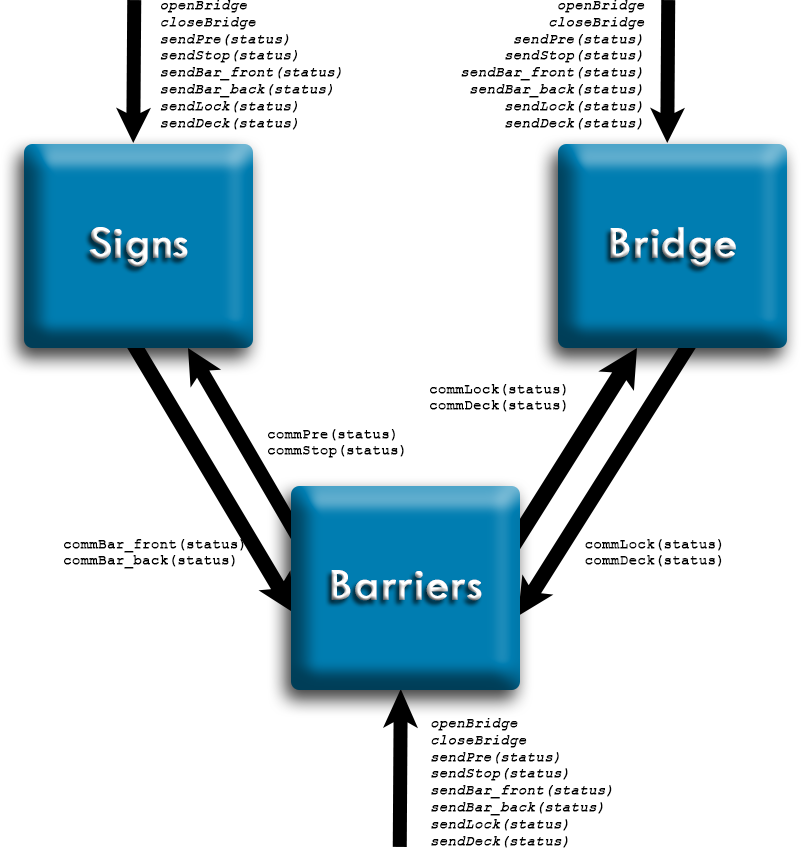
\includegraphics[width=0.5\columnwidth]{Images/Architecture}%
\caption{Communication flow between parallel processes \emph{signs}, \emph{barriers} and \emph{bridge}.}%
\label{fig:arch}%
\end{figure}
%

\newpage

\section{Translation of Requirements in Terms of Interactions}
\label{sec:trans}

In order to create a model for the bridge in mCRL2, which is a modeling software used for system validation, the requirements have to expressed in terms of the previous stated interactions. Then, in order to check our model in mCRL2, the requirements have to be written using $\mu$-calculus. During the project, these translations will be used for model checking.

Because the requirements often concern all individual objects of a specific component (sign or barrier), the variables $i, j$ have been introduced. When discussing signs, these variables will satisfy $i,j \in \{$1,2,3,4$\}$. For example, parameter \texttt{S$_i$} in the $\mu$-calculus covers all four stop signs being S$_1$, S$_2$, S$_3$ and S$_4$. When discussing barriers or locks, $i,j \in \{$1,2$\}$ holds and \texttt{L$_i$} in the $\mu$-calculus covers both locks being L$_1$ and L$_2$.
%
\begin{enumerate}
  \setcounter{enumi}{-1}

  %Example
  \item \textbf{Example; B cannot happen unless A happened first.}
  \begin{enumerate}
		\item Only when action \texttt{A} has occurred first, action \texttt{B} can occur.
		\item $[true^* \cdot \overline{A}^{*} \cdot B]false$
	\end{enumerate}

	%Requirement 1
	\item \textbf{Stop signs cannot be switched on unless all pre lights are switched on}
	\begin{enumerate}
		\item Always after a \texttt{commPre($P_i$, off)}, a \texttt{cSwitchStop($S_j$, on)} cannot occur unless \texttt{cSwitchPre($P_j$, on)} has occurred intermediately for all $P_j$.
		\item $[true^* \cdot commPre(P_i, off) \cdot \overline{cSwitchPre(P_i, on)}^{*} \cdot cSwitchStop(S_j, on)]false$
	\end{enumerate}

	%Requirement 2
	\item \textbf{Barriers cannot be lowered unless all stop signs are switched on}
	\begin{enumerate}
		\item Always after a \texttt{commStop(S$_i$, off)}, a \texttt{cFrontBarrier($B_j$, down)} or \texttt{cBackBarrier($B_j$, down)} cannot occur unless a \texttt{cStopSign($S_i$, on)} has occurred intermediately.
		\item $[true^* \cdot commStop(S_i, off) \cdot \overline{cSwitchStop(S_i, on)}^{*} \cdot (cFrontBarrier(B_j, lower) \vee cBackBarrier(B_j, lower))]false$ \\
	\end{enumerate}

	%Requirement 3
	\item \textbf{The first barrier to be encountered by the cars is lowered earlier than the second in order to enable cars to leave the bridge}
	\begin{enumerate}
		\item Always when \texttt{cBackBarrier($B_i$, lower)}, \texttt{cFrontBarrier($B_i$, lower)} has to be occurred before. No \texttt{cFrontBarrier($B_i$, lift)} may have occurred intermediately.
		\item $[true^* \cdot commFrontBarrier(B_i, up) \cdot \overline{cFrontBarrier(B_i, down)}^{*} \cdot cBackBarrier(B_i, down)]false$\\
	\end{enumerate}

	%Requirement 4
	\item \textbf{The bridge can only be unlocked when all barriers are down}
	\begin{enumerate}
		\item Always after a \texttt{commFrontBarrier($B_i$, lift)}, \texttt{cLock($L_j$, disengage)} cannot occur unless a \texttt{cFrontBarrier($B_i$, lower)} has occurred intermediately. \\
					Always after a \texttt{commBackBarrier($B_i$, lift)}, \texttt{cLock($L_j$, disengage)} cannot occur unless a \texttt{cBackBarrier($B_i$, lower)} has occurred intermediately.
		\item $[true^* \cdot commFrontBarrier(B_i, lift) \cdot \overline{cFrontBarrier(B_i, lower)}^{*} \cdot cLock(L_j, disengaged)]false$
					$[true^* \cdot commBar\_front(B_i, lift) \cdot \overline{cBackBarrier(B_i, lower)}^{*} \cdot cLock(L_j, disengaged)]false$
	\end{enumerate}

	%Requirement 5
	\item	\textbf{The deck can only be lifted when both locks are disengaged}
	\begin{enumerate}
		\item Always after a \texttt{commLock($L_i$, engaged)}, a \texttt{cDeck(up)} cannot occur unless a \texttt{cLock($L_i$, disengaged)} has occurred for all $L_i$ intermediately.
		\item $[true^* \cdot commLock(L_i, engaged)\cdot \overline{cLock(L_i, disengaged)}^{*} \cdot cDeck(up)]false$\\
	\end{enumerate}

	%Requirement 6
	\item \textbf{Bridge locks can only be engaged when the deck is down}
	\begin{enumerate}
		\item Always when \texttt{cLock($L_i$, engaged)} then \texttt{cDeck(down)} has occurred before, and no \texttt{commDeck(up)} has occurred intermediately.
		\item $[true^* \cdot commDeck(up) \cdot \overline{cDeck(down)}^{*} \cdot cLock(L_i, engaged)]false$\\
	\end{enumerate}

	%Requirement 7
	\item \textbf{Barriers can only be up when the bridge is locked by the locks}
	\begin{enumerate}
		\item Always after a \texttt{commLock($L_i$, disengaged)}, a \texttt{cFrontBarrier($B_j$, lift)} or \texttt{cBackBarrier($B_j$, lift)} cannot occur unless a \texttt{cLock($L_i$, engaged)} has occurred intermediately.
		\item $[true^* \cdot commLock(L_i, disengaged)\cdot \overline{cLock(L_i, engage)}^{*} \cdot (cBackBarrier(B_j, lift) \vee cFrontBarrier(B_j, lift))]false$\\
	\end{enumerate}

	%Requirement 8
	\item \textbf{Stop signs can only be shut off only when all barriers are up}
	\begin{enumerate}
		\item Always when cSwitchOff($S_j$, off) occurs, \texttt{cFrontBarrier($B_i$, lift)} and \texttt{cBackBarrier($B_i$, lift)} have to be occurred and no \texttt{cFrontBarrier($B_i$, lower)} or \texttt{cBackBarrier($B_i$, lower)} may have occurred intermediately.
		\item $[true^* \cdot commFrontBarrier(B_i, lower) \cdot \overline{cFrontBarrier(B_i, lift)}^{*} \cdot cSwitchStop(S_j, off)]false$
					$[true^* \cdot commBackBarrier(B_i, lower) \cdot \overline{cBackBarrier(B_i, lift)}^{*} \cdot cSwitchStop(S_j, off)]false$
	\end{enumerate}

	%Requirement 9
	\item \textbf{The bridge should be able to be opened when a ship approaches}
	\begin{enumerate}
		\item From every state eventually \texttt{cDeck(up)} can occur.
		\item $[true^*]<true^* \cdot cDeck(up)>true$
	\end{enumerate}

	%Requirement 10
	\item \textbf{The bridge should be able to close in order to let cars pass}
	\begin{enumerate}
		\item From every state eventually \texttt{cSwtichStop(off)} can occur.
		\item $[true^*]<true^* \cdot cSwitchStop(S_i, off)>true$
	\end{enumerate}

	%Requirement 11
	\item \textbf{If the motor is in the 'broken' status, the may not be moved up or down.}
	\begin{enumerate}
		\item Always after a \texttt{motorStatus(broken)}, a \texttt{cDeck(lift)} or \texttt{cDeck(lower)} cannot happen unless a \texttt{motorStatus(!broken)} happened intermediately.
		\item $[true^* \cdot motorStatus(Broken) \cdot \overline{motorStatus(\neg Broken)^*}  \cdot (cDeck(up) \vee cDeck(down))]false$
	\end{enumerate}

\end{enumerate}


\section{Modeling the Bridge Using mCRL2}
\label{sec:model}

With the requirements clearly stated, now the bridge can be modeled. In order to create a model that can be verified using $\mu$-calculus, the mCRL2 program can be used. The code for the model can be found in \ref{sec:mcrl} or the attached file \texttt{Bridge\_group7.mcrl2}. Section \ref{sec:basic} describes the first steps towards the model, declaring the data structs, actions and processes for the . The implementation of the safety layer is discussed second, in section \ref{sec:safety}. Section \ref{sec:ids} will finally explain the introduction of component identities.

\subsection{Setting up the Basic Structure}
\label{sec:basic}
When writing the code, we kept to the architecture from section \ref{sec:act} including three component processes (\emph{Signs}, \emph{Barriers} and \emph{Bridge}). As explained in section \ref{sec:act}, five data structures are introduced to group possible states of the component. These are to be found at the beginning of the code. Next, each process is preceded by an \texttt{act}-section holding all interactions that apply to that particular process. By creating this structure, it is easy to see which interactions belong to which process. The processes themselves are pretty simple. The can basically perform two actions:
%
\begin{itemize}
	\item send their status towards the safety layer by means of a \texttt{send} action
	\item confirm an execution action of the safety layer by means of a \texttt{r}-action
\end{itemize}
%
All multi-actions (\texttt{comm} for the status update and \texttt{c} for execution) are synchronized in the \texttt{comm}-section at the bottom of the code. This section, which is part of the \texttt{init}-section, also holds all commands that the bridge operator can perform. These can be found in the \texttt{allow}-part. Finally, all processes are assigned an initial state and separated by two bars ($||$), indicating parallel execution. 

\subsection{Adding the Safety Layer}
\label{sec:safety}
Since there is not yet a safety layer to block dangerous commands, all possible transitions can be taken. Locks can be disengaged without stop signs being switched on first, decks could be opened while the barriers are still up etc. Creating the fourth process (the \emph{Safety layer}) has been a quite time-consuming step. Every command that is in the \texttt{allow}-part, is first checked for safety in the safety layer by looking at its adjacent components (see table \ref{tab:open} and \ref{tab:close}). The structure of the can be compared with \texttt{if}-loops, since actions can be performed only if the requirements are satisfied. With the implementation of the safety layer, two types of transitions exist:
%
\begin{itemize}
	\item node-to-node transitions, only taken when considered to be safe
	\item self-loops, containing actions that are considered unsafe or meaningless (e.g. switching on the stop signs when the deck is lifted, while a lifted deck already implies switched on stop signs)
\end{itemize}
%
Figure \ref{fig:global} shows a general overview made with \texttt{lts$\_$graph}. Here the node-to-node transitions can be seen as the connection between groups of states, which represent the nodes. The self-loop transitions are the reason for the cluttered groups of states, since many actions end up being a self-loop.
%
\begin{figure}[htb]
\centering
\includegraphics[width=\columnwidth]{Images/global_graph.pdf}
\caption{Graphical representation of the model, showing the global strucuture of the system.}%
\label{fig:global}
\end{figure}%
%
\subsection{Separating Components into Individual Objects}
\label{sec:ids}
Finally, the abstract components are assigned an  identity as a second parameter, this way creating unique instances of the components. As you can imagine, the safety layer will expand because of this. A simple check whether the barriers are down, now becomes four checks for barrier B1, B2, B3 and B4, respectively. Since the identities of the components can also be grouped, four new data structures have been added at the beginning of the code. With respect to the usability of the system, we have decided not to implement the identities in the global interactions. Thus, the bridge operator can only control the components all together. This prevent the bridge operator to have a \texttt{setLock(disengage)} command being blocked because of three lowered barriers, while the operator himself under the presumption all barriers are down. Expanding the user interface with control to individual objects requires a well-designed user interface and the provision of helpful feedback by the safety layer. Since these are not in the scope of this project, we have decided to keep the global interactions general. Figure \ref{fig:detailed} shows a section of \texttt{lts$\_$graph}, depicting all transitions leaving and entering the pre sign node. This image is applicable to all nodes from figure \ref{fig:global}.
%
\begin{figure}[htb]
\centering
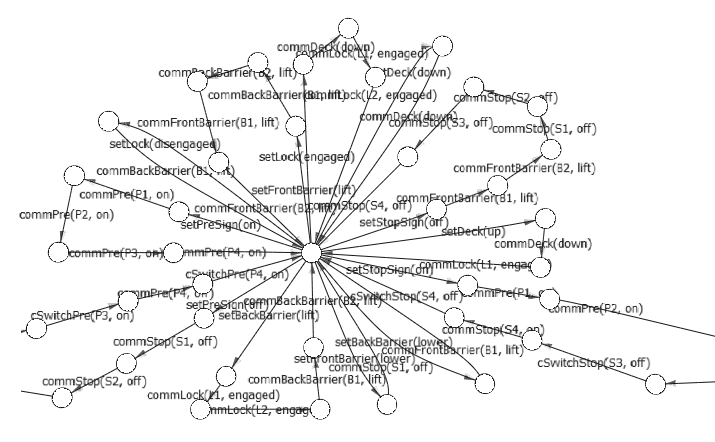
\includegraphics[width=\columnwidth]{Images/detail_graph_gebeund.png}
\caption{Detailed representation of the model (pre sign node), depicting the check procedures for all possible commands.}%
\label{fig:detailed}
\end{figure}%
%

\newpage
\section{Checks}

Bla

\section{Conclusion and Discussion}
In this Report we find that that the model that is made in MCRL2 is succesfully verified by our requirements. Futher improvement to the MRCL2 model is still to be made in order to get more control over every bridge component.


%----------------------------------------------------------------------------------------
%	Appendices
%----------------------------------------------------------------------------------------
\newpage
\appendix

\section{Model of the Bridge: mCRL2 Code}
\label{sec:mcrl}

%\lstinputlisting{Bridge_group7.txt}

\section{MCF Files}

\label{sec:mcf}

\subsection{check01.mcf}
\lstinputlisting[style=custommcrl2]{mcrl2/checks/check01.mcf}

\subsection{check02.mcf}
\lstinputlisting[style=custommcrl2]{mcrl2/checks/check02.mcf}

\subsection{check03.mcf}
\lstinputlisting[style=custommcrl2]{mcrl2/checks/check03.mcf}

\subsection{check04.mcf}
\lstinputlisting[style=custommcrl2]{mcrl2/checks/check04.mcf}

\subsection{check05.mcf}
\lstinputlisting[style=custommcrl2]{mcrl2/checks/check05.mcf}

\subsection{check06.mcf}
\lstinputlisting[style=custommcrl2]{mcrl2/checks/check06.mcf}

\subsection{check07.mcf}
\lstinputlisting[style=custommcrl2]{mcrl2/checks/check07.mcf}

\subsection{check08.mcf}
\lstinputlisting[style=custommcrl2]{mcrl2/checks/check08.mcf}

\subsection{check09.mcf}
\lstinputlisting[style=custommcrl2]{mcrl2/checks/check09.mcf}

\subsection{check10.mcf}
\lstinputlisting[style=custommcrl2]{mcrl2/checks/check10.mcf}

\subsection{check11.mcf}
\lstinputlisting[style=custommcrl2]{mcrl2/checks/check11.mcf}


%----------------------------------------------------------------------------------------
%	BIBLIOGRAPHY
%----------------------------------------------------------------------------------------
%
%\bibliographystyle{unsrt}
%
%\bibliography{sample}
%
%----------------------------------------------------------------------------------------

\end{document}



